\documentclass[letterpaper,10pt]{article}

%\setlength{\parindent}{0in}
%\usepackage{fullpage} 
\usepackage{amsmath}
\usepackage{amssymb}
\usepackage{enumerate}
\usepackage{graphicx}
\usepackage[table]{xcolor}
\usepackage{dcolumn}
\oddsidemargin 0.0in
\textwidth 6.5in
\newcolumntype{.}{D{.}{.}{-1}}
\newcommand*{\myalign}[2]{\multicolumn{1}{#1}{#2}}

\title{Final Exam}
\author{Steve Mazza}
\date{December 18, 2011}

\begin{document}
\maketitle
In all cases please consult the accompanying spreadsheet for clarification of the calculations.

\begin{enumerate}
% QUESTION 1
\item % DONE
Using ordinary least squares regression I calculate the following key values:
\begin{center}
\begin{tabular}{l.}
\hline
&\myalign{l}{\textbf{Coefficients}} \\
\hline
Intercept & -20.86713 \\
Sorties & 0.51197 \\
Experience & -0.51064 \\
\hline
\end{tabular}
\end{center}

I then calculate the predicted monthly cost of Unscheduled Maintenance Actions as follows:
\begin{align*}
\mbox{Monthly Cost} &= 5\times \$1,000\times (-20.86713 + 30\times 0.51197 + 3\times -0.51064) \\
&= \$5,000\times (-20.86713 + 15.3591 - 1.5319) \\
&= \$5,000\times 7.0399 \\
&= \$35,199.65
\end{align*}

Please see the accompanying spreadsheet for justification.

% QUESTION 2
\item % DONE
Using the data provided, a first missile production unit could be estimated at \$5.2M using the Wright learning curve approach as follows:
	\begin{align*}
	2,500,000 &= a10^{\left(\frac{\log_{10}.8}{\log_{10}2}\right)} \\
	2,500,000 &= 0.47651a \\
	a &\approx 5.24648\times 10^{6} \\
	a &\approx 5,246,480
	\end{align*}
	
% QUESTION 3
\item % DONE
The COCOMO II model was used with the following inputs:
	\begin{itemize}
	\item Required Development Schedule: LOW
	\item SW Required Reliability: HIGH
	\item Language and Toolset Experience: HIGH
	\item Platform Volatility: LOW
	\item Use of Software Tools: VERY HIGH
	\item \% Design Modified: 20
	\item \% Code Modified: 33
	\item \% Integration Required: 67
	\item \% Assessment and Assimilation: 2
	\item \% Software Understanding: $(30+30+20)/3 \approx 27$
	\item Unfamiliarity: 1
	\end{itemize}
For the basis of calculation I used \$10K per person-month as the cost for the software engineering effort.
%\begin{table}[htdp]
\begin{center}
\begin{tabular}{rrrrrrr}
\hline
\myalign{c}{\textbf{Month}} & \myalign{c}{\textbf{Inception}} & \myalign{c}{\textbf{Elaboration}} & \myalign{c}{\textbf{Construction}} & \myalign{c}{\textbf{Transition}} & \myalign{c}{\textbf{Hardware}} & \myalign{c}{\textbf{Monthly Total}} \\
\hline
1&  \$183,883.25 &&&& \$145,735.56 & \$329,618.81  \\
2&  \$183,883.25 &&&& \$145,735.56 & \$329,618.81  \\
3&  \$183,883.25 &&&& \$145,735.56 & \$329,618.81  \\
4&  \$183,883.25 &&&& \$145,735.56 & \$329,618.81  \\
5&& \$245,177.67 &&& \$145,735.56 & \$390,913.22   \\
6&& \$245,177.67 &&& \$145,735.56 & \$390,913.22  \\
7&& \$245,177.67 &&& \$145,735.56 & \$390,913.22  \\
8&& \$245,177.67 &&& \$145,735.56 & \$390,913.22  \\
9&& \$245,177.67 &&& \$145,735.56 & \$390,913.22  \\
10&& \$245,177.67 &&& \$145,735.56 & \$390,913.22  \\
11&& \$245,177.67 &&& \$145,735.56 & \$390,913.22  \\
12&& \$245,177.67 &&& \$145,735.56 & \$390,913.22  \\
13&& \$245,177.67 &&& \$145,735.56 & \$390,913.22  \\
14&& \$245,177.67 &&& \$145,735.56 & \$390,913.22  \\
15&& \$245,177.67 &&& \$145,735.56 & \$390,913.22  \\
16&& \$245,177.67 &&& \$145,735.56 & \$390,913.22  \\
17&&& \$465,838 && \$145,735.56 & \$611,573.06  \\
18&&& \$465,838 && \$145,735.56 & \$611,573.06  \\
19&&& \$465,838 && \$145,735.56 & \$611,573.06  \\
20&&& \$465,838 && \$145,735.56 & \$611,573.06  \\
21&&& \$465,838 && \$145,735.56 & \$611,573.06  \\
22&&& \$465,838 && \$145,735.56 & \$611,573.06  \\
23&&& \$465,838 && \$145,735.56 & \$611,573.06  \\
24&&& \$465,838 && \$145,735.56 & \$611,573.06  \\
25&&& \$465,838 && \$145,735.56 & \$611,573.06  \\
26&&& \$465,838 && \$145,735.56 & \$611,573.06  \\
27&&& \$465,838 && \$145,735.56 & \$611,573.06  \\
28&&& \$465,838 && \$145,735.56 & \$611,573.06  \\
29&&& \$465,838 && \$145,735.56 & \$611,573.06  \\
30&&& \$465,838 && \$145,735.56 & \$611,573.06  \\
31&&& \$465,838 && \$145,735.56 & \$611,573.06  \\
32&&& \$465,838 && \$145,735.56 & \$611,573.06  \\
33&&& \$465,838 && \$145,735.56 & \$611,573.06  \\
34&&& \$465,838 && \$145,735.56 & \$611,573.06  \\
35&&& \$465,838 && \$145,735.56 & \$611,573.06  \\
36&&& \$465,838 && \$145,735.56 & \$611,573.06  \\
37&&&& \$367,766.50 && \$367,766.50 \\
38&&&& \$367,766.50 && \$367,766.50 \\
39&&&& \$367,766.50 && \$367,766.50 \\
40&&&& \$367,766.50 && \$367,766.50 \\
\hline
&&&&&\textbf{Grand Total:} & \textbf{\$19,711,961.00}
\end{tabular}
\end{center}
%\end{table}

% QUESTION 4
\item %I have answers for this but am not confident on part b.  For 1 point I'm not going to worry about it just yet.
	\begin{enumerate}
	\item The \emph{uniform} distribution applies in this case as the description is taken almost exactly from the definition.
	\item While this appears to be somewhat \emph{normal}, there is a strong indication that the Nominal values will prevail.  On the other hand, this does not appear to be so clear as to be represented by a \emph{triangle} distribution.  It is possible that the most appropriate model here is the \emph{lognormal} distribution.
	\item This probabilities in this case are most appropriately represented by the \emph{normal} distribution.
	\item Since there appears to be a most likely value, the \emph{triangle} distribution would apply here.
	\end{enumerate}
	
% QUESTION 5
\item % DONE
The COSYSMO model was used with the following inputs:
	\begin{itemize}
	\item System Size
		\begin{itemize}
		\item 30 easy requirements
		\item 60 nominal requirements
		\item 40 difficult requirements
		\item 6 nominal interfaces
		\item 6 difficult interfaces
		\item 15 nominal algorithms
		\item 5 difficult algorithms
		\item 3 nominal operational scenarios
		\item 1 difficult operational scenario
		\end{itemize}
		\item Requirements Understanding: LOW
		\item Process Capability: HIGH
		\item Personnel Experience: HIGH
		\item Labor Cost: \$10,000 per person-month
	\end{itemize}
	
The graph below indicates the resulting confidence levels.
	\begin{center}
	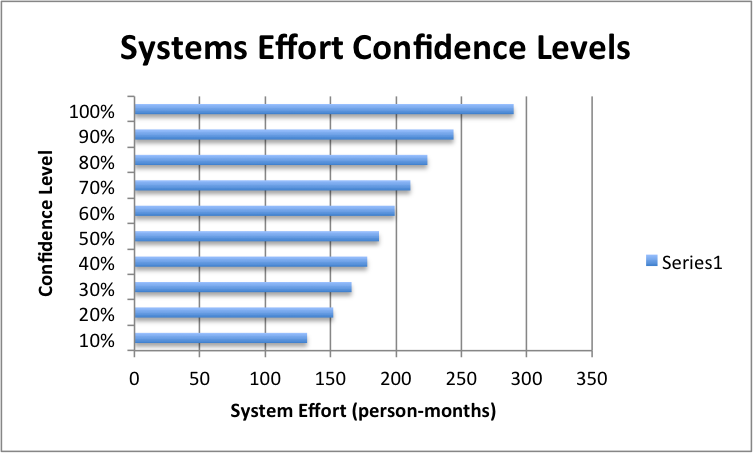
\includegraphics[scale=.75]{picture0.png}
	\end{center}

The calculations indicate that my Command can assume an approximately 15\% probability of achieving the contractor's bid.  

A 70\% confidence level estimate for actual budgeting and risk reserve would be met within a 211 person-months, or \$2,110,000.00.

% QUESTION 6
\item % DONE
Using the formula supplied,
	\[
	\mbox{Effort (Person-Months)} = 0.25\times\mbox{System Requirements}^{1.06}
	\]
I calculate the original cost without process improvement to be 181.5 person-months or \$1,814,881.25.  Using the modified formula,
	\[
	\mbox{Effort (Person-Months)} = 0.25\times\mbox{System Requirements}^{1.03}
	\]
I calculate the new cost with the process improvement to be 150.6 person-months or \$1,506,187.76 for a savings of 30.9 person-months or \$308,693.49 annually.

The 5-year Return On Investment (ROI) is calculated to be \$5.17 for each dollar spent as follows:
	\begin{align*}
	\mbox{ROI} &= (5\times\mbox{Savings} - \mbox{Costs}) / \mbox{Costs} \\
	&=  (5\times \$308,693.49 - \$250,000.00) / \$250,000.00 \\
	&= (\$1,543,467.45 - \$250,000.00) / \$250,000.00 \\
	&= \$1,293,467.45 / \$250,000.00 \\
	&= \$5.17
	\end{align*}

% QUESTION 7
\item % DONE
The results are based on the following adjustments to the System Cost Drivers:
\begin{center}
\begin{tabular}{lll}
\hline
& \textbf{COA 1} & \textbf{COA 2} \\
\hline
Technology Risk & High & Nominal \\
System Level of Service Requirements & Low & Nominal \\
Requirements Understanding & High & Nominal \\
Number of Recursive Levels in the System Design & Low & Nominal \\
System Architecture Understanding & High & Nominal \\
\hline
\end{tabular}
\end{center}
Note that I used a value of High for the Technology Risk.  The three criteria you gave us did not agree so I assumed that the Risk would necessarily be equivalent to the worst case.

Please see the accompanying spreadsheet for an explanation of the calculations.  A summary of the annual costs follows:
\begin{center}
\begin{tabular}{rrr}
\hline
& \myalign{c}{\textbf{COA 1}} & \myalign{c}{\textbf{COA 2}} \\
\hline
FY12 & \$2,050,459.57 & \$2,878,384.40 \\
FY13 & \$2,603,993.60 & \$1,649,750.54 \\
FY14 & \$4,347,253.04 & \$2,386,694.82 \\
FY15 & \$3,945,656.47 & \$1,218,426.92 \\
FY16 & \$2,740,866.75 & \$1,112,220.75 \\
FY17 & \$2,740,866.75 & \$1,112,220.75 \\
\hline
\end{tabular}
\end{center}
I was tempted to assume that, ``�the years FY12 to FY17,'' is a 60-month period but decided to include FY17 calculations as well just to be safe.  Please omit FY17 numbers (which are maintenance only) if this is not what you intended.
\end{enumerate}
\end{document}